
Comparing predictive models across diffusion MRI studies remains challenging.
Preprocessing pipelines differ substantially, microstructural information is represented in multiple ways (e.g., voxel-wise maps, 
ROI summaries, or learned embeddings), and evaluation protocols vary in data splits, cross-validation schemes, and hyperparameter selection.
As a result, reported performance differences may reflect methodological inconsistencies rather than genuine modeling improvements.
Limited code and configuration sharing further restrict reproducibility.
Together, these factors make it difficult to determine which approaches generalize reliably and provide meaningful insights.
To address these issues, we introduce a standardized benchmark that unifies preprocessing and feature extraction, evaluates both 
classical and deep learning models on regression and classification tasks, and spans multiple public datasets under a 
controlled evaluation protocol.
We now describe the benchmark in detail whose overall structure is illustrated in Figure~\ref{fig:benchmark_overview}.

\begin{figure}[htbp]
    \centering
    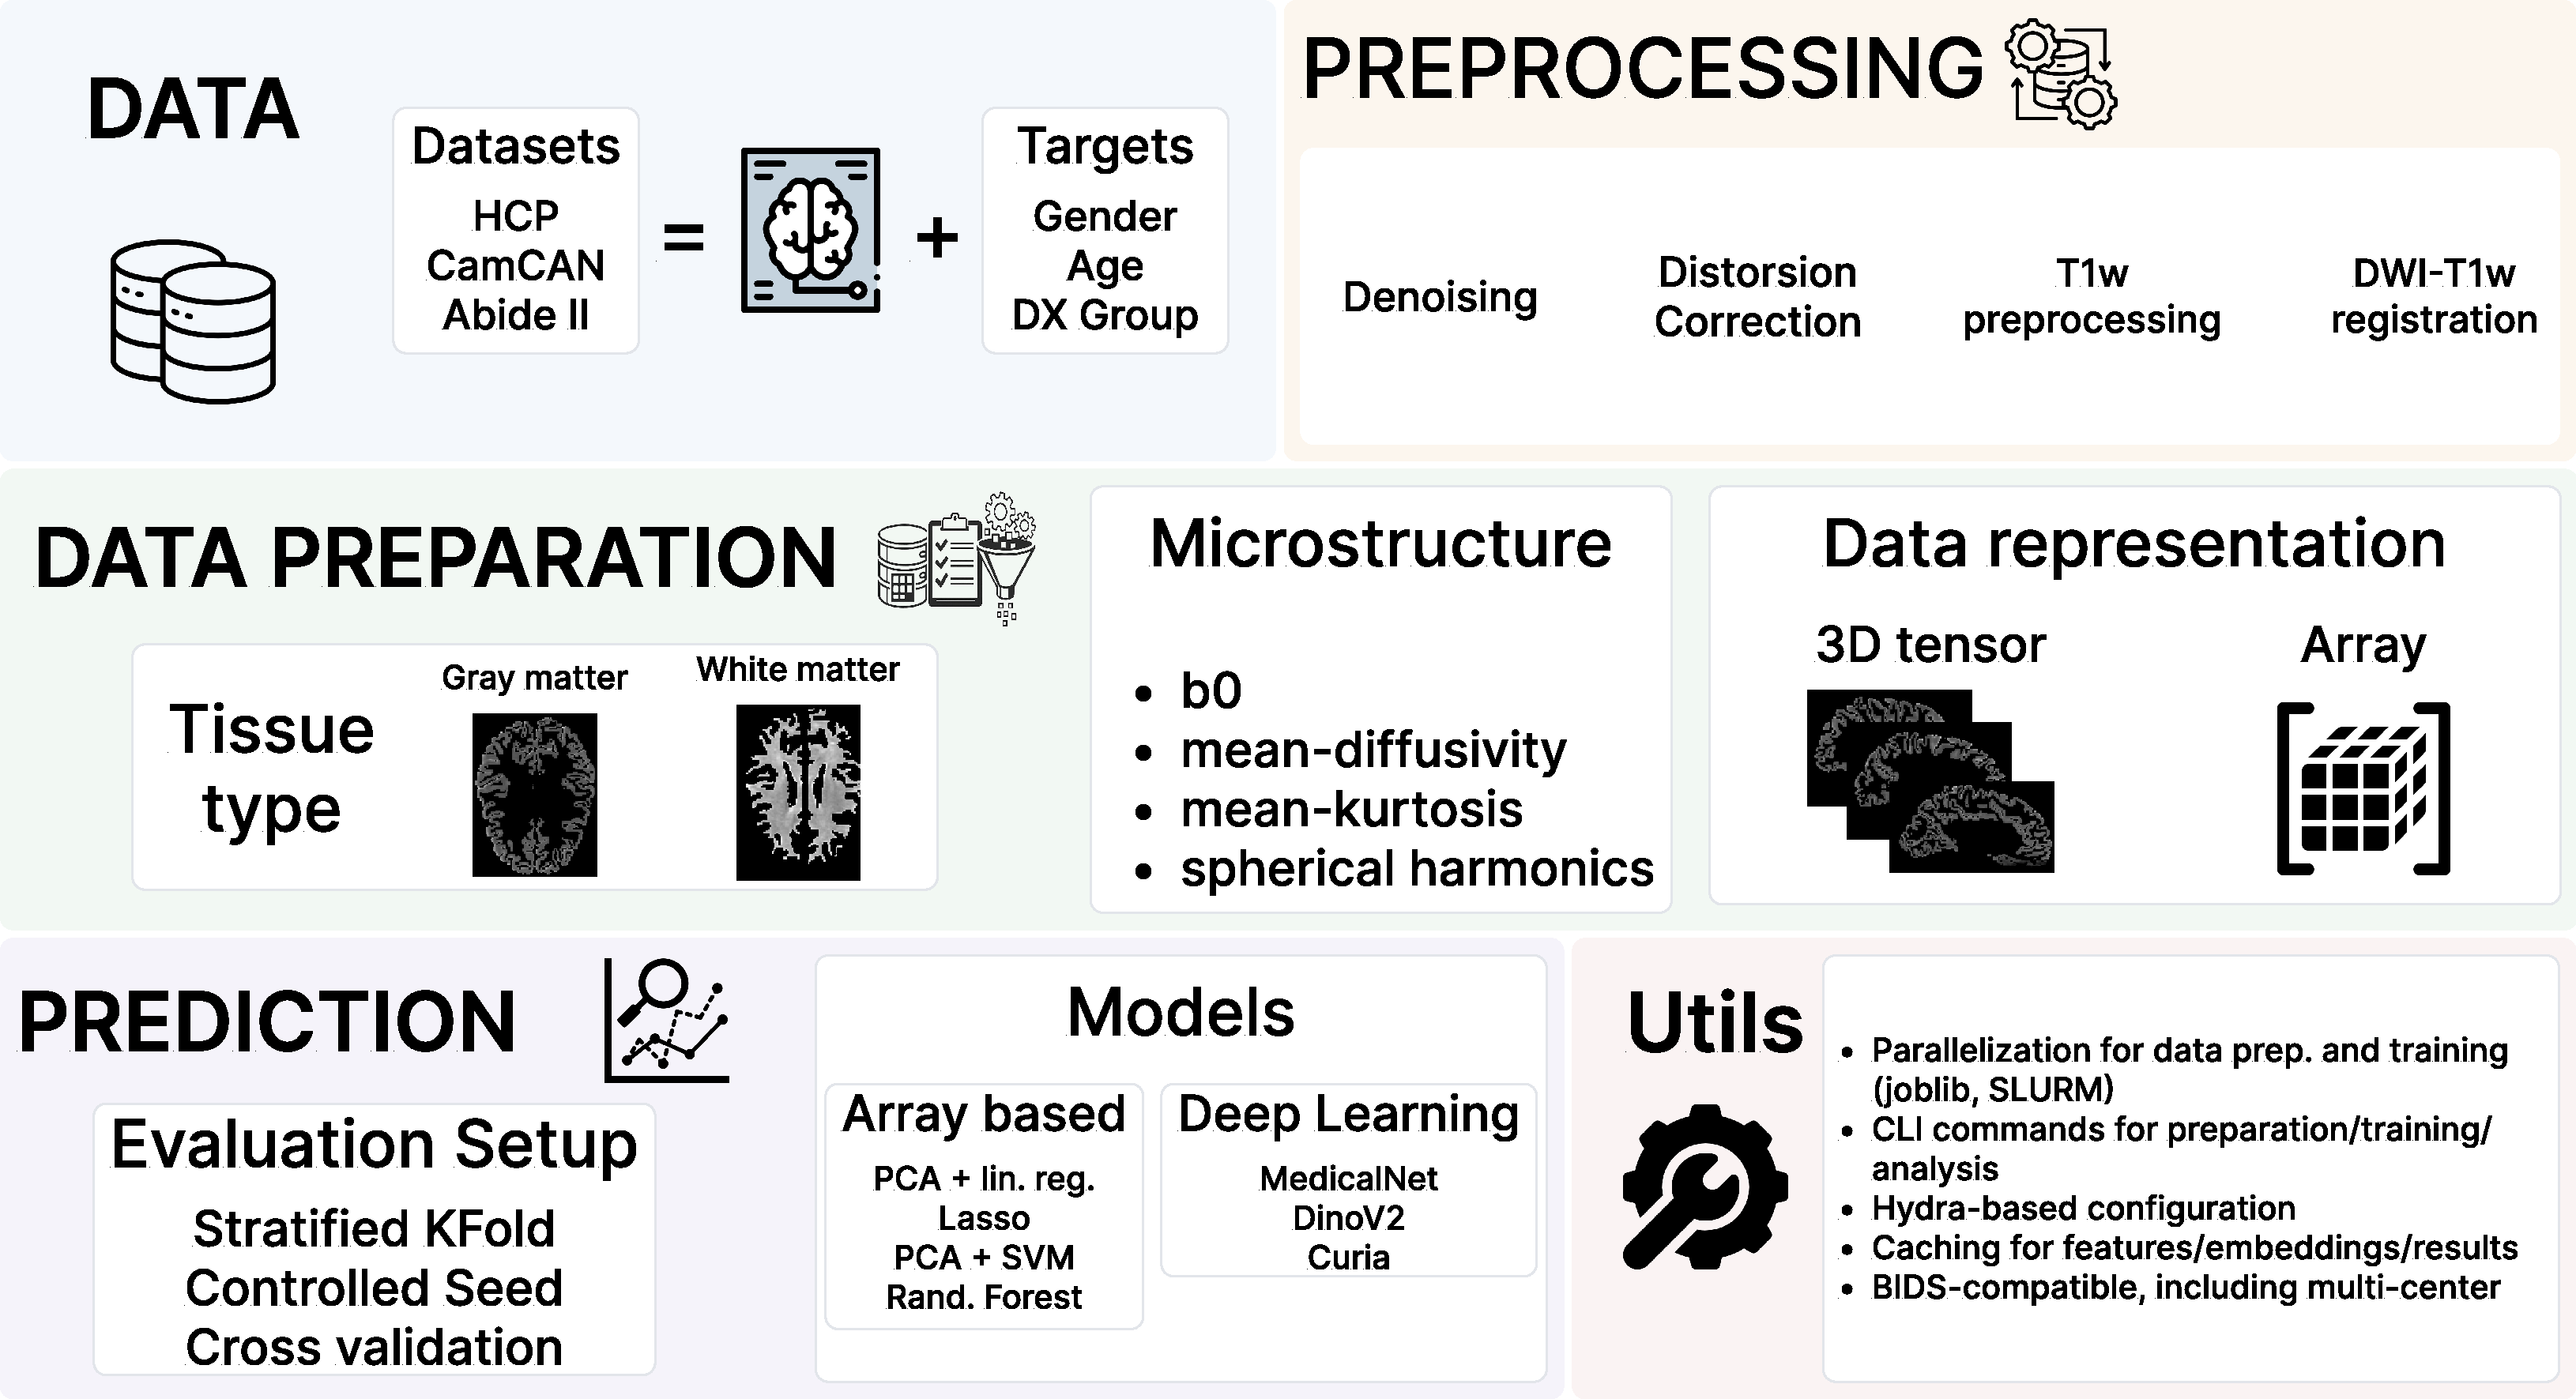
\includegraphics[width=\textwidth]{scheme.pdf}
    \caption{Overview of the proposed diffusion MRI benchmark pipeline, illustrating the end-to-end 
    process from preprocessing to microstructural feature extraction, predictive modeling, and 
    evaluation.}
    \label{fig:benchmark_overview}
\end{figure}

\subsection{Datasets}
    
% \begin{itemize}
%     \item Introduction sentence about why you picked these datasets
%     \item Introduce Number of subjects
%     \item Age range / demographics
%     \item Scanner details
%     \item Acquisition protocol or summary table with acquisition parameters
%     \item Prediction targets (classification/regression)
% \end{itemize}
To ensure reproducibility, we evaluate our benchmark on three publicly available datasets 
covering both healthy and clinical populations.
\textbf{HCP}: The Human Connectome Project (HCP) Young Adult dataset \cite{van2013wu} targets gender and age. It includes 
1,036 healthy subjects after filtering (474 males, 562 females; ages 22-37).
HCP data were acquired on a customized Siemens 3T Connectome scanner using a multi-shell Spin-Echo EPI sequence 
(TR/TE = 5520/89.5 ms, 1.25 mm isotropic, multiband factor 3; $b$-values = 1000, 2000, 3000 s/mm$^2$, 90 directions/shell).
\textbf{Cam-CAN}: The Cambridge Centre for Ageing and Neuroscience (Cam-CAN) dataset \cite{shafto2014cambridge} targets 
gender and age. It includes 629 healthy subjects (316 males, 313 females; ages 18-88), scanned on a Siemens 3T TIM Trio using 
a 2D twice-refocused SE EPI sequence (TR/TE = 9100/104 ms, 2.0 mm isotropic; $b$-values = 1000, 2000 s/mm$^2$, 30 directions each).
\textbf{ABIDE II}: The Autism Brain Imaging Data Exchange II (ABIDE II) dataset \cite{di2017enhancing} targets Autism Spectrum 
Disorder (ASD) diagnosis.
It includes 218 subjects (186 males, 32 females; ages 5-64), including 119 with ASD and 99 controls.
As a multi-site dataset, ABIDE II data were acquired on various 3T scanners with highly heterogeneous, site-specific 
single-shell diffusion protocols.
Across the included sites, spatial resolutions range from 0.94 to 3.0 mm, TR/TE from 5200-20244/78-101 ms, $b$-values include 
1000, 1500, and 2500 s/mm$^2$, and diffusion directions vary between 32 and 64.
This variability provides a realistic scenario for evaluating model robustness to scanner heterogeneity.

% \begin{table*}[htbp]
%     \centering
%     \caption{Diffusion MRI acquisition parameters for HCP and Cam-CAN datasets.}
%     \label{tab:acquisition_params}
%     \begin{tabular}{lccccccccc}
%         \toprule
%         \textbf{Dataset} & \textbf{Sequence} & \textbf{TR/TE (ms)} & \textbf{Res. (mm)} & \textbf{FOV (mm)} & \textbf{Slices} & \textbf{$b$-values (s/mm$^2$)} & \textbf{Dirs.} & \textbf{Echo Sp. (ms)} & \textbf{MB} \\
%         \midrule
%         \textbf{HCP} & SE EPI & 5520 / 89.5 & 1.25 iso & 210$\times$180 & 111 & 1000, 2000, 3000 & 90/shell & 0.78 & 3 \\
%         \textbf{Cam-CAN} & 2D SE EPI & 9100 / 104 & 2.0 iso & 192$\times$192 & 66 & 1000, 2000 & 30 & 0.72 & - \\
%         \bottomrule
%     \end{tabular}
% \end{table*}

% If space (unlikely):
% * PLOTS: Demographic distribution (age histograms) | Table with demographics summary (gender classes, age range...)

\subsection{Data Preparation}
\subsubsection{Preprocessing}
% \begin{itemize}
%     \item Denoising
%     \item Motion and eddy correction
%     \item Spatial normalization
%     \item Masking strategy
% \end{itemize}
Except for the HCP dataset, which has its own preprocessing pipeline,
the DWI data were preprocessed using the diffusion-preprocessing package\footnote{\url{https://github.com/man-shu/diffusion-preprocessing}} which containerizes 
several other software dependencies such as dipy \cite{Garyfallidis2014}, sMRIPrep\footnote{\url{https://github.com/nipreps/smriprep}}, FSL \cite{Smith2004}, 
ANTs \cite{Avants2009}, FreeSurfer \cite{Dale1999} and AFNI \cite{Cox1996}.
%
The images were first denoised using the \emph{Marchenko-Pastur} PCA method (MPPCA) \cite{Veraart2016a,Cordero-Grande2019} implemented with
dipy's \emph{dipy\_denoise\_mppca} function.
%
This denoising procedure identifies the principal components corresponding to noise and then removes them from the DWI data \cite{Veraart2016a}.
%
After MPPCA denoising, Gibbs ringing artifacts \cite{Veraart2016b} were also removed using dipy's \emph{dipy\_gibbs\_ringing} function.
%
Next, to correct the distortions due to inhomogeneities of the magnetic field, FSL's eddy correction \cite{Andersson2016} was used.
%
Then this denoised and distortion-corrected DWI data were registered to the anatomical T1w image using FreeSurfer's \emph{bbregister} 
function \cite{greve2009accurate} with 12 degrees of freedom and boundary-based registration cost function.
%
The anatomical T1w image was preprocessed using sMRIPrep \url{https://github.com/nipreps/smriprep}.

\subsubsection{Spatial normalization}
% Explain here the different forms of input representation.
% The word "feature representation" is ambigiuous because neural network also extract features in a data-driven way. That's why I would rather use the term like "Microstructural Representation".
% Explain why differences between white and gray matter. Give references here about why there are differences.
% %%%%%%%%%%%%%%
% To capture the distinct properties of the brain, we extract specific inputs for gray and 
% white matter. We use the term ``microstructural representation'' rather than ``feature representation'' 
% to clearly distinguish our explicitly computed biological metrics from the latent features learned 
% data-drivenly by neural networks. Gray and white matter exhibit fundamentally different diffusion 
% profiles due to their distinct cellular architectures—gray matter being rich in cell bodies and 
% dendrites, while white matter consists primarily of myelinated axonal tracts \cite{jones2010diffusion, 
% basser1994mr}. Consequently, we employ tailored extraction strategies for each tissue type using our 
% automated preprocessing pipeline.

\paragraph{Gray Matter}
% \todo{Refs}
Gray matter microstructure was represented on the subject-specific cortical surface reconstructed from 
T1-weighted images using the Desikan–Killiany atlas (aparc). For each subject, cortical meshes 
(white/pial surfaces) were generated and diffusion-derived scalar maps
were computed in native diffusion space and rigidly aligned to the anatomical space. Voxelwise 
diffusion measures were then projected onto the individual cortical surface using ribbon-constrained 
sampling, preserving vertex-wise resolution (~64k vertices per hemisphere) \cite{greve2009accurate}. This subject-specific 
surface representation was chosen to respect cortical geometry, reduce partial-volume effects, and 
maintain high spatial specificity while enabling anatomically consistent regional correspondence via 
the atlas labels across subjects.
    % \begin{itemize}
    %     \item Voxel-wise features
    %     \item High-dimensional representation (~64k features)
    %     \item Mask-based extraction
    % \end{itemize}
    % Explain that voxel-wise features preserve spatial resolution but increase dimensionality and risk of overfitting.

\paragraph{White Matter}
White matter microstructure was represented within a standardized tract space using the Tract-Based 
Spatial Statistics (TBSS) framework \cite{smith2006tract}. Diffusion-derived scalar maps were nonlinearly registered to 
standard space, projected onto the group-wise white matter skeleton to minimize partial volume effects 
and residual misalignment, and summarized using the JHU White-Matter Tractography Atlas \cite{mori2008stereotaxic}. Mean 
microstructural values were extracted from 48 major bundles defined in the atlas, yielding a compact 
tract-level representation per metric. We intentionally adopted this skeleton-based, atlas-constrained 
strategy rather than subject-specific tractography to enforce anatomical correspondence across subjects,
 reduce variability introduced by tracking parameters, and enhance robustness in a multi-dataset 
 benchmarking setting. Although this representation sacrifices voxel-level granularity relative to the 
 cortical surface analysis, it provides reproducible, homologous bundle definitions across datasets and
  mitigates registration and tract delineation inconsistencies—thereby strengthening cross-cohort 
  comparability and methodological stability.


% White matter microstructure was summarized within a common tract space using a predefined tract 
% dictionary derived from a standardized atlas-based segmentation (e.g., 48 major bundles). Diffusion 
% scalar maps were computed voxelwise in native space and projected onto a template skeleton to ensure 
% anatomical correspondence across subjects. For each tract, mean microstructural values were extracted, 
% yielding a compact 48-dimensional representation per metric. This tract-averaged template-based 
% strategy was selected to ensure cross-subject anatomical consistency, reduce variability arising from 
% subject-specific tractography, and improve robustness in a benchmarking setting. Although this results 
% in lower dimensionality compared to the vertex-wise cortical representation, it provides stable, 
% reproducible white matter features aligned to homologous bundles across datasets.

    % \begin{itemize}
    %     \item Tract-based aggregation
    %     \item Mean values per tract (~48 features)
    %     \item Reduced dimensionality
    %     \item Anatomical interpretability
    % \end{itemize}
    % Justify tract-averaged representation: Noise reduction, improved stability, lower dimensional feature space, anatomically meaningful structure


\subsubsection{Microstructural representation}
To capture the biological properties of brain tissue, we compute a diverse set of 
microstructural metrics using established diffusion models. These metrics were selected to represent 
different facets of tissue architecture, ranging from basic diffusion magnitude to complex restricted 
environments:
\begin{itemize}
    \item \textbf{Baseline ($b=0$):} The averaged T2-weighted non-diffusion signal is included as a 
    baseline to disentangle purely diffusion-driven predictive power from underlying structural T2 
    contrast.
    \item \textbf{Mean Diffusivity (MD):} Computed via Diffusion Tensor Imaging (DTI) \cite{basser1994mr}, representing 
    the overall magnitude of water diffusion.
    \item \textbf{Mean Kurtosis (MK):} Derived from Diffusion Kurtosis Imaging (DKI) \cite{jensen2005diffusional}, capturing the 
    non-Gaussianity of diffusion as a proxy for microstructural heterogeneity and tissue complexity.
    % \item \textbf{Return-To-Origin Probability (RTOP):} Estimated using a Laplacian-regularized Mean 
    % Apparent Propagator (MAP-MRI) model. RTOP reflects the probability of water molecules remaining in 
    % their initial position, serving as a strong indicator of cellular restriction and density.
    \item \textbf{Spherical Harmonics (SH) Power:} A model-free representation obtained by computing the 
    L2 norm of the SH coefficients \cite{tournier2004direct} (up to order 6) directly from the diffusion signal, capturing signal 
    complexity and anisotropy without assuming a specific tissue compartment model.
    % \item \textbf{Spherical Harmonics (SH) Power:} A model-free metric computed by least-squares 
    % projection of the b0-normalized signal $S(\mathbf{g})/S_0$ onto a real, symmetric SH basis 
    % ($\ell_{\max}{=}6$, 28 coefficients; Descoteaux~\textit{et al.}~\shortcite{descoteaux2007regularized} 
    % convention, \texttt{sf\_to\_sh} in DiPy~\shortcite{garyfallidis2014dipy}). The scalar is the 
    % $\ell_2$ norm $\|\mathbf{c}\|_2$, capturing angular complexity without any compartment model.
\end{itemize}
% To mitigate scanner-specific scaling effects and harmonize data across multi-site cohorts 
% (e.g., ABIDE II), 
We apply a ventricular normalization strategy to avoid the effect of free water in the signal \cite{pasternak2009free}. For each subject, 
voxel-wise diffusion metrics are divided by the mean metric value extracted from the cerebrospinal 
fluid (ventricles). Finally, extreme pathological values are clipped at the 99th percentile to ensure 
numerical stability during model training.

    % \begin{itemize}
    %     \item Binary targets (encoded 0/1), Continuous targets (standardized during training)
    %     \item Standardization fitted on training set only
    %     \item Applied to validation/test sets 
    %     \item Inverse transform for regression outputs (for visualization)
    % \end{itemize}

\subsection{Prediction models}
Our benchmark includes a wide 
spectrum of predictive models, ranging from linear baselines to advanced deep 
learning architectures. We first compare linear models 
(e.g., logistic regression, Lasso), Random Forests, and Support Vector Machines 
(SVM) \cite{hastie2009elements}. Given the high dimensionality of the microstructural representations, we 
also evaluate these models coupled with Principal Component Analysis (PCA) for 
feature reduction. 

We also benchmark several vision architectures. We leverage 
pre-trained models, specifically DINOv2 \cite{oquab2023dinov2} and Curia \cite{dancette2025curia}, utilizing them as 
frozen feature extractors where representations are computed offline prior to 
training the prediction head. In contrast, the smaller 3D architecture MedicalNet \cite{chen2019med3d} is 
fine-tuned on our diffusion datasets to adapt to the specific 
microstructural domains. 
% The applied prediction head is an MLP with two hidden layers (512 and 128 units) and ReLU 
% activations, trained using the Adam optimizer with a learning rate of 1e-4 and early stopping based on validation 
% performance.
% \begin{itemize}
%     \item Dummy baseline (e.g., majority class for classification, mean predictor for regression)
%     \item Classical ML pipeline: Linear models (e.g., logistic regression, linear regression), Random Forests, Support Vector Machines (SVM) + their PCA versions
%     \item Deep Learning models (e.g., dinov2, medicalnet)
%     \item Unified hyperparameter search strategy (e.g., grid search or random search with cross-validation on the training set)
% \end{itemize}

\subsection{Benchmarks tasks and evaluation metrics}
% Task selection rationale: Clinical relevance, data availability, and established benchmarks in the literature.
The selection of prediction tasks in our benchmark is driven by clinical relevance, data availability, 
and the need to align with established benchmarks in the neuroimaging literature. We evaluate models 
across two primary paradigms:

\subsubsection{Classification} 
For binary classification, we focus on tasks such as Autism Spectrum Disorder (ASD) diagnosis (ASD vs. 
Typically Developing) using the ABIDE II dataset, as well as gender prediction in the HCP and Cam-CAN 
cohorts. We report performance using balanced accuracy, taking into account class imbalances.


% \begin{itemize}
%     \item Task description: Binary diagnosis prediction (e.g., ASD vs. TD)
%     \item Evaluation Metrics: Accuracy, AUC, F1-score
% \end{itemize}

\subsubsection{Regression} 
We evaluate brain age estimation using the healthy cohorts from Cam-CAN. 
We report performance using R² and MAE.

% \begin{itemize}
%     \item Task description: Age prediction (brain age estimation)
%     \item Evaluation Metrics: R², MAE
% \end{itemize}

\subsection{Evaluation protocols}
To rigorously evaluate the predictive models, we employ a stratified 5-fold cross-validation strategy. 
We also ensure fixed and reproducible splits through seed initialization. Strict 
separation between training and testing data is maintained at all stages; preprocessing steps, feature 
normalization, and hyperparameter tuning are fitted exclusively on the training set of each fold and 
subsequently applied to the held-out test set, preventing any information leakage. 

% \begin{itemize}
%     \item Data Splitting Strategy (Fixed train/test splits)
%     \item Cross-validation within training set. Stratification
%     \item No information leakage
%     \item Mean ± std across folds
%     \item Statistical comparison tests (e.g., paired t-tests, Wilcoxon signed-rank tests) to assess significance of performance differences between models
% \end{itemize}

%%%%%%%%%%%
% \subsection{Prediction}
% \begin{itemize}
%     \item Feature normalization
%         \begin{itemize}
%             \item Binary targets (encoded 0/1), Continuous targets (standardized during training)
%             \item Standardization fitted on training set only
%             \item Applied to validation/test sets 
%             \item Inverse transform for regression outputs (for visualization)
%         \end{itemize}
%     \item Task definitions and labels and reasons for task selection
%         \begin{itemize}
%             \item Classification: Binary diagnosis prediction (e.g., ASD vs. TD)
%             \item Regression: Age prediction (brain age estimation)
%             \item Task selection rationale: Clinical relevance, data availability, and established benchmarks in the literature
%         \end{itemize}
%     \item Evaluation Metrics
%         \begin{itemize}
%             \item Classification: Accuracy, AUC, F1-score
%             \item Regression: R², MAE
%             \item Mean ± std across folds
%             \item Statistical comparison tests (e.g., paired t-tests, Wilcoxon signed-rank tests) to assess significance of performance differences between models
%         \end{itemize}
%     \item Models Used
%         \begin{itemize}
%             \item Dummy baseline (e.g., majority class for classification, mean predictor for regression)
%             \item Classical ML pipeline: Linear models (e.g., logistic regression, linear regression), Random Forests, Support Vector Machines (SVM) + their PCA versions
%             \item Deep Learning models (e.g., dinov2, medicalnet)
%             \item Unified hyperparameter search strategy (e.g., grid search or random search with cross-validation on the training set)
%         \end{itemize}
% \end{itemize}

% \subsection{Validation, Evaluation and Visualizations}
% \begin{itemize}
%     \item Data Splitting Strategy (Fixed train/test splits)
%     \item Cross-validation within training set. Stratification
%     \item No information leakage
%     \item Explanation of plots and statistics
% \end{itemize}